\documentclass[tikz,border=0pt]{standalone}
\usepackage{fontspec}
\usepackage{xcolor}
\definecolor{ink}{HTML}{17243A}
\definecolor{muted}{HTML}{637086}
\definecolor{grid}{HTML}{E3E7ED}
\definecolor{rho}{HTML}{2C7A7B}
\definecolor{b2}{HTML}{78909C}
\definecolor{four}{HTML}{C58B2A}
\definecolor{b3}{HTML}{B94949}
\setmainfont{DejaVu Sans}
\begin{document}
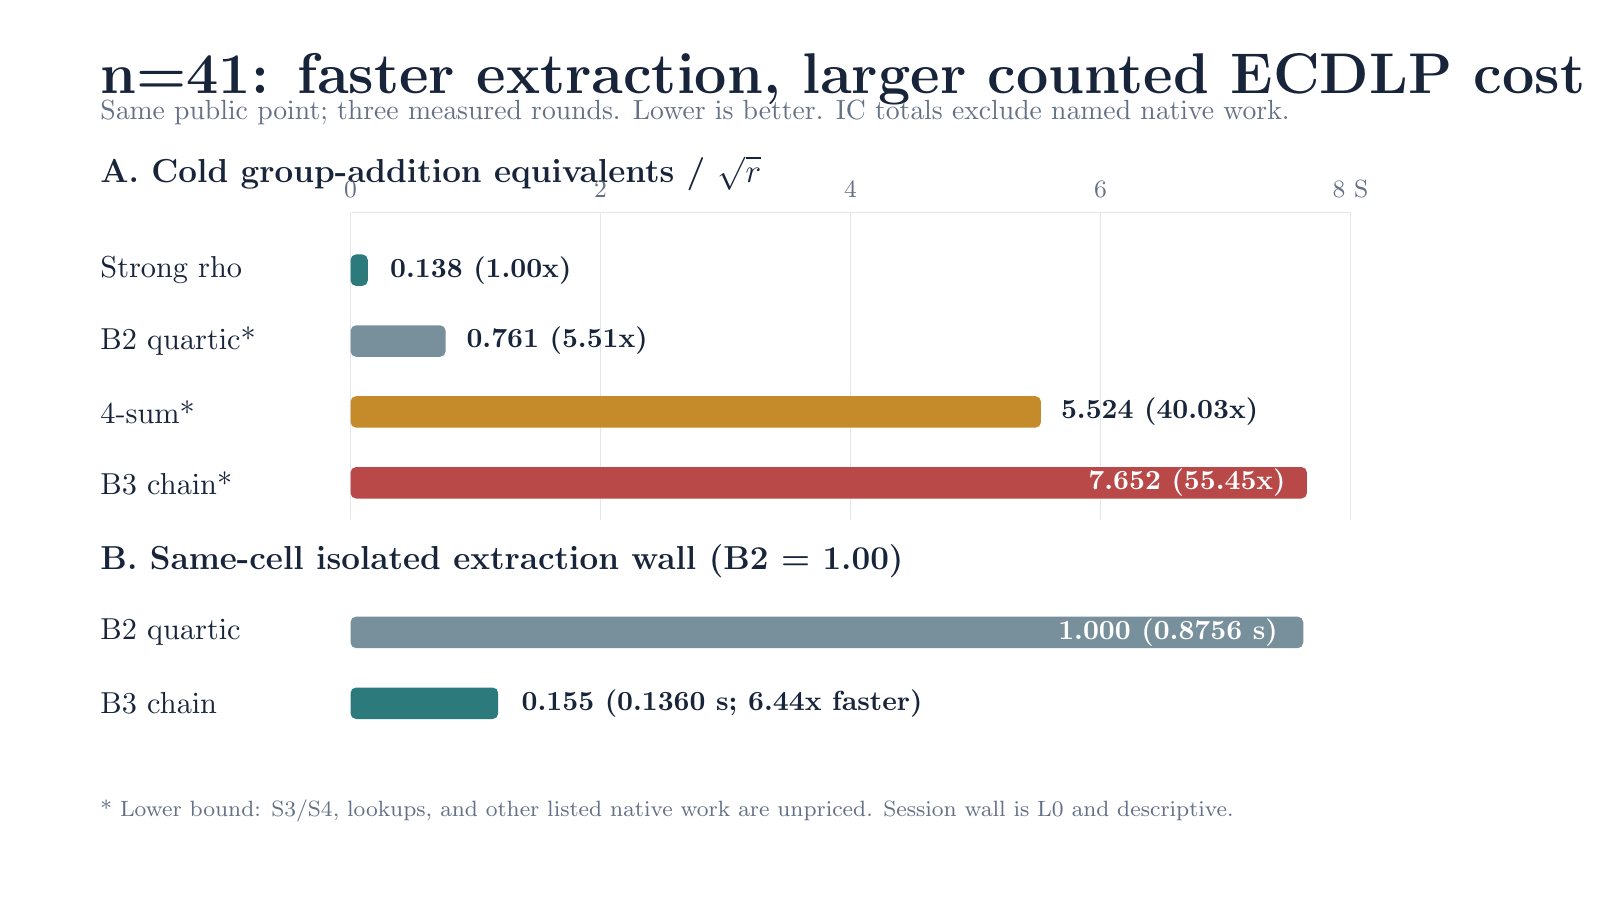
\begin{tikzpicture}[x=1cm,y=1cm]
  \fill[white] (0,0) rectangle (18,10.8);
  \node[anchor=west,text=ink,font=\bfseries\fontsize{20}{22}\selectfont] at (0.8,10.15) {n=41: faster extraction, larger counted ECDLP cost};
  \node[anchor=west,text=muted,font=\fontsize{10}{12}\selectfont] at (0.8,9.72) {Same public point; three measured rounds. Lower is better. IC totals exclude named native work.};
  \node[anchor=west,text=ink,font=\bfseries\fontsize{13}{15}\selectfont] at (0.8,8.95) {A. Cold group-addition equivalents / $\sqrt{r}$};
  \draw[grid] (4.1,8.45) -- (16.8,8.45);
  \foreach \x/\lab in {4.1/0,7.275/2,10.45/4,13.625/6,16.8/8 S} {
    \draw[grid] (\x,8.45) -- (\x,4.55);
    \node[anchor=south,text=muted,font=\fontsize{9}{10}\selectfont] at (\x,8.52) {\lab};
  }
  \foreach \y/\lab in {7.72/Strong rho,6.82/B2 quartic*,5.92/4-sum*,5.02/B3 chain*} {
    \node[anchor=west,text=ink,font=\fontsize{11}{12}\selectfont] at (0.8,\y) {\lab};
  }
  \fill[rho,rounded corners=2pt] (4.1,7.52) rectangle (4.32,7.92);
  \fill[b2,rounded corners=2pt] (4.1,6.62) rectangle (5.308,7.02);
  \fill[four,rounded corners=2pt] (4.1,5.72) rectangle (12.869,6.12);
  \fill[b3,rounded corners=2pt] (4.1,4.82) rectangle (16.247,5.22);
  \node[anchor=west,text=ink,font=\bfseries\fontsize{10}{11}\selectfont] at (4.48,7.72) {0.138 (1.00x)};
  \node[anchor=west,text=ink,font=\bfseries\fontsize{10}{11}\selectfont] at (5.45,6.82) {0.761 (5.51x)};
  \node[anchor=west,text=ink,font=\bfseries\fontsize{10}{11}\selectfont] at (13.0,5.92) {5.524 (40.03x)};
  \node[anchor=east,text=white,font=\bfseries\fontsize{10}{11}\selectfont] at (16.1,5.02) {7.652 (55.45x)};
  \node[anchor=west,text=ink,font=\bfseries\fontsize{13}{15}\selectfont] at (0.8,4.02) {B. Same-cell isolated extraction wall (B2 = 1.00)};
  \node[anchor=west,text=ink,font=\fontsize{11}{12}\selectfont] at (0.8,3.12) {B2 quartic};
  \node[anchor=west,text=ink,font=\fontsize{11}{12}\selectfont] at (0.8,2.22) {B3 chain};
  \fill[b2,rounded corners=2pt] (4.1,2.92) rectangle (16.2,3.32);
  \fill[rho,rounded corners=2pt] (4.1,2.02) rectangle (5.976,2.42);
  \node[anchor=east,text=white,font=\bfseries\fontsize{10}{11}\selectfont] at (16.0,3.12) {1.000 (0.8756 s)};
  \node[anchor=west,text=ink,font=\bfseries\fontsize{10}{11}\selectfont] at (6.15,2.22) {0.155 (0.1360 s; 6.44x faster)};
  \node[anchor=west,text=muted,font=\fontsize{8.5}{10}\selectfont] at (0.8,0.85) {* Lower bound: S3/S4, lookups, and other listed native work are unpriced. Session wall is L0 and descriptive.};
\end{tikzpicture}
\end{document}
